\documentclass[border=5mm]{standalone}
\usepackage[utf8]{inputenc}
\usepackage[T1]{fontenc}
\usepackage{tikz}
\usepackage{inconsolata}
\usetikzlibrary{calc}

\begin{document}
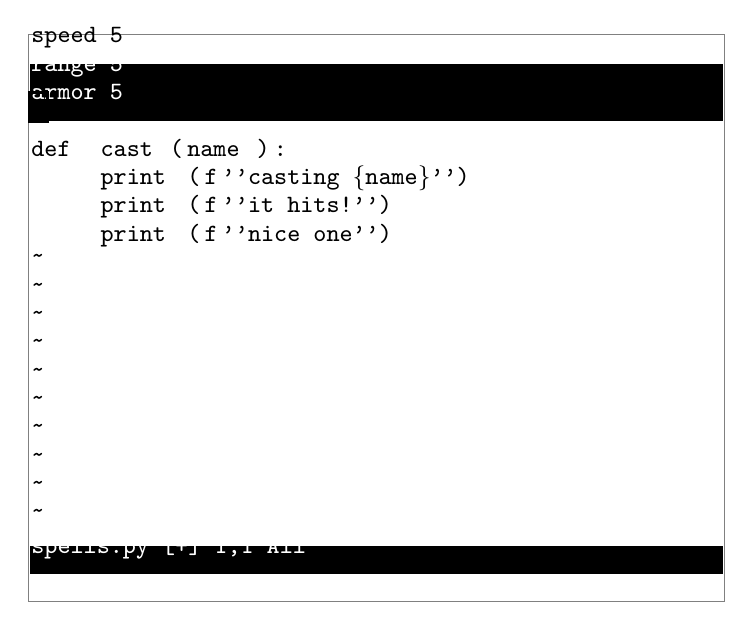
\begin{tikzpicture}[x=\dimexpr 0.22cm, y=\dimexpr 0.36cm]

  \draw[gray, thin] (-0.1, 0.3) rectangle (40.1, -19.7);

  \fill[black] (0, -0.75) rectangle (40, -1.75);
  \fill[black] (0, -1.75) rectangle (40, -2.75);
  \fill[black] (0, -17.75) rectangle (40, -18.75);

  \node[anchor=base west, inner sep=0pt, font=\ttfamily\small] at (0.05, 0) {speed 5};
  \node[anchor=base west, text=white, inner sep=0pt, font=\ttfamily\small] at (0.05, -1) {range 5};
  \node[anchor=base west, text=white, inner sep=0pt, font=\ttfamily\small] at (0.05, -2) {armor 5};
  \node[anchor=base west, inner sep=0pt, font=\ttfamily\small] at (0.05, -4) {def};
  \node[anchor=base west, inner sep=0pt, font=\ttfamily\small] at (4.05, -4) {cast};
  \node[anchor=base west, inner sep=0pt, font=\ttfamily\small] at (8.05, -4) {(};
  \node[anchor=base west, inner sep=0pt, font=\ttfamily\small] at (9.05, -4) {name};
  \node[anchor=base west, inner sep=0pt, font=\ttfamily\small] at (13.05, -4) {)};
  \node[anchor=base west, inner sep=0pt, font=\ttfamily\small] at (14.05, -4) {:};
  \node[anchor=base west, inner sep=0pt, font=\ttfamily\small] at (4.05, -5) {print};
  \node[anchor=base west, inner sep=0pt, font=\ttfamily\small] at (9.05, -5) {(};
  \node[anchor=base west, inner sep=0pt, font=\ttfamily\small] at (10.05, -5) {f};
  \node[anchor=base west, inner sep=0pt, font=\ttfamily\small] at (11.05, -5) {''casting \{name\}'')};
  \node[anchor=base west, inner sep=0pt, font=\ttfamily\small] at (4.05, -6) {print};
  \node[anchor=base west, inner sep=0pt, font=\ttfamily\small] at (9.05, -6) {(};
  \node[anchor=base west, inner sep=0pt, font=\ttfamily\small] at (10.05, -6) {f};
  \node[anchor=base west, inner sep=0pt, font=\ttfamily\small] at (11.05, -6) {''it hits!'')};
  \node[anchor=base west, inner sep=0pt, font=\ttfamily\small] at (4.05, -7) {print};
  \node[anchor=base west, inner sep=0pt, font=\ttfamily\small] at (9.05, -7) {(};
  \node[anchor=base west, inner sep=0pt, font=\ttfamily\small] at (10.05, -7) {f};
  \node[anchor=base west, inner sep=0pt, font=\ttfamily\small] at (11.05, -7) {''nice one'')};
  \node[anchor=base west, inner sep=0pt, font=\ttfamily\small] at (0.05, -8) {\~{}};
  \node[anchor=base west, inner sep=0pt, font=\ttfamily\small] at (0.05, -9) {\~{}};
  \node[anchor=base west, inner sep=0pt, font=\ttfamily\small] at (0.05, -10) {\~{}};
  \node[anchor=base west, inner sep=0pt, font=\ttfamily\small] at (0.05, -11) {\~{}};
  \node[anchor=base west, inner sep=0pt, font=\ttfamily\small] at (0.05, -12) {\~{}};
  \node[anchor=base west, inner sep=0pt, font=\ttfamily\small] at (0.05, -13) {\~{}};
  \node[anchor=base west, inner sep=0pt, font=\ttfamily\small] at (0.05, -14) {\~{}};
  \node[anchor=base west, inner sep=0pt, font=\ttfamily\small] at (0.05, -15) {\~{}};
  \node[anchor=base west, inner sep=0pt, font=\ttfamily\small] at (0.05, -16) {\~{}};
  \node[anchor=base west, inner sep=0pt, font=\ttfamily\small] at (0.05, -17) {\~{}};
  \node[anchor=base west, text=white, inner sep=0pt, font=\ttfamily\small] at (0.05, -18) {spells.py [+]         1,1            All};
  \draw[black, very thick] (0, -1.75) rectangle (1, -2.75);

\end{tikzpicture}
\end{document}